\documentclass[../main.tex]
		
		\begin{document}
			\begin{description}
		\item[Task:] Understand subobjects of a graph.
		\item[Definition:] Let $(V, E)$ and $(V', E')$ be graphs. The graph $(V', E')$ is called a subgraph of $(V, E)$ if $V' \subseteq V$ and $E' \subseteq E$, \textbf{i.e.} if $(V', E')$ consists of a subset $V'$ of the vertices of $(V, E)$ and a subset $E'$ of edges $(V, E)$ between vertices in $V'$.
		\item[Example:] Star of David on the flag of Israel \\
			$V = \{a, b, c, d, e, f\}$ \\
			$E = \{ac, ce, ae, bf, fd, bd\}$ \\
			\begin{figure}[h!]
				\centering
				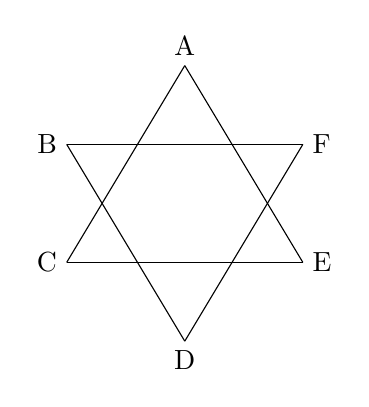
\begin{tikzpicture}
				\coordinate (A) at (0, 0);
				\coordinate (B) at (-1.5, -1);
				\coordinate (C) at (-1.5, -2.5);
				\coordinate (D) at (0, -3.5);
				\coordinate (E) at (1.5, -2.5);
				\coordinate (F) at (1.5, -1);
				
				\draw (A) node[above]{A} -- (C);
				\draw (A) -- (E) node[right]{E};
				\draw (C) node[left]{C} -- (E);
				\draw (D) -- (B) node[left]{B};
				\draw (D) node[below]{D} -- (F);
				\draw (B) -- (F) node[right]{F};
			\end{tikzpicture}
		\end{figure}
		\item 2 triangle subgraphs of the star of David: \\
		\begin{tabular}{ll}
				$V' = \{a, c, e\}$ & $E' = \{ac, ce, ae\}$ \\
				$V'' = \{b, f, d\}$ & $E'' = \{bf, fd, bd\}$
		\end{tabular}
	\end{description}
	

\end{document}